\documentclass[tikz,border=3pt]{standalone}
\usepackage{times}
\usepackage{amsmath,amssymb}
\usepackage{siunitx}
\usepackage{graphicx}
\usepackage{pgfplots}
\pgfplotsset{compat=1.18}
\usepgfplotslibrary{groupplots,fillbetween,colorbrewer}
\usetikzlibrary{arrows.meta,positioning,calc,fit,backgrounds,shapes.geometric,decorations.pathreplacing,patterns,matrix}
\graphicspath{{../}{../figures/}}
\definecolor{cmpc}{HTML}{C0392B}
\definecolor{csch}{HTML}{1F5FA8}
\definecolor{cstk}{HTML}{6E6E6E}
\definecolor{cband}{HTML}{F4C7C3}
\definecolor{crec}{HTML}{2B2B2B}
\definecolor{cphase}{HTML}{FBE3C2}
\newlength{\pw}\newlength{\ph}
\pgfplotsset{
  paperaxis/.style={scale only axis, tick label style={font=\scriptsize}, label style={font=\footnotesize}, title style={font=\footnotesize, yshift=-1mm},
    legend style={font=\scriptsize, draw=black!25, fill=white, legend cell align=left, /tikz/every even column/.append style={column sep=6pt}}, axis line style={black!60}, tick style={black!60}, every axis plot/.append style={line width=0.9pt},
    grid=major, grid style={black!12}, xlabel near ticks, ylabel near ticks, ylabel shift=-2pt, xlabel shift=-2pt, clip marker paths=true},
}
\newcommand{\panel}[2]{\node[anchor=north west, font=\footnotesize\bfseries, inner sep=1.5pt, fill=white, fill opacity=0.85, text opacity=1] at (rel axis cs:0.015,0.985) {(#1)#2};}
\newcommand{\gth}{g_\theta}
\newcommand{\thsp}{\theta_{\mathrm{sp}}}

\pgfplotsset{discard if not/.style 2 args={x filter/.append code={\edef\tempa{\thisrow{#1}}\edef\tempb{#2}\ifx\tempa\tempb\else\def\pgfmathresult{inf}\fi}}}

\definecolor{mSWE}{HTML}{D6E4F5}\definecolor{mPIA}{HTML}{FCE3C8}\definecolor{mBPH}{HTML}{D9EFD3}\definecolor{mLSM}{HTML}{F6D0CC}\definecolor{mPLT}{HTML}{E8E8E8}
\definecolor{bLin}{HTML}{4A78B5}\definecolor{bLN}{HTML}{8E7CC3}\definecolor{bAtt}{HTML}{E08A2E}\definecolor{bFFN}{HTML}{3C9D6A}\definecolor{bPhy}{HTML}{2C7FB8}\definecolor{bQP}{HTML}{C0392B}\definecolor{bTok}{HTML}{F1C40F}
\tikzset{
  mod/.style={draw=black!40, rounded corners=5pt, fill=#1, inner sep=0pt},
  modtitle/.style={font=\footnotesize\bfseries, anchor=north west, inner sep=4pt},
  blk/.style={draw=#1, fill=#1!15, rounded corners=2pt, font=\scriptsize, minimum height=5.2mm, inner sep=3pt, align=center},
  tok/.style={draw=black!50, fill=bTok!60, minimum width=3.4mm, minimum height=6.5mm, inner sep=0pt},
  ctx/.style={draw=black!60, fill=bAtt!50, minimum width=3.8mm, minimum height=6.5mm, inner sep=0pt, font=\tiny},
  arr/.style={-{Latex[length=1.8mm]}, line width=0.6pt, black!70},
  farr/.style={-{Latex[length=2.4mm]}, line width=1.1pt, black!80},
  note/.style={font=\scriptsize, align=left, inner sep=1pt},
}
\begin{document}
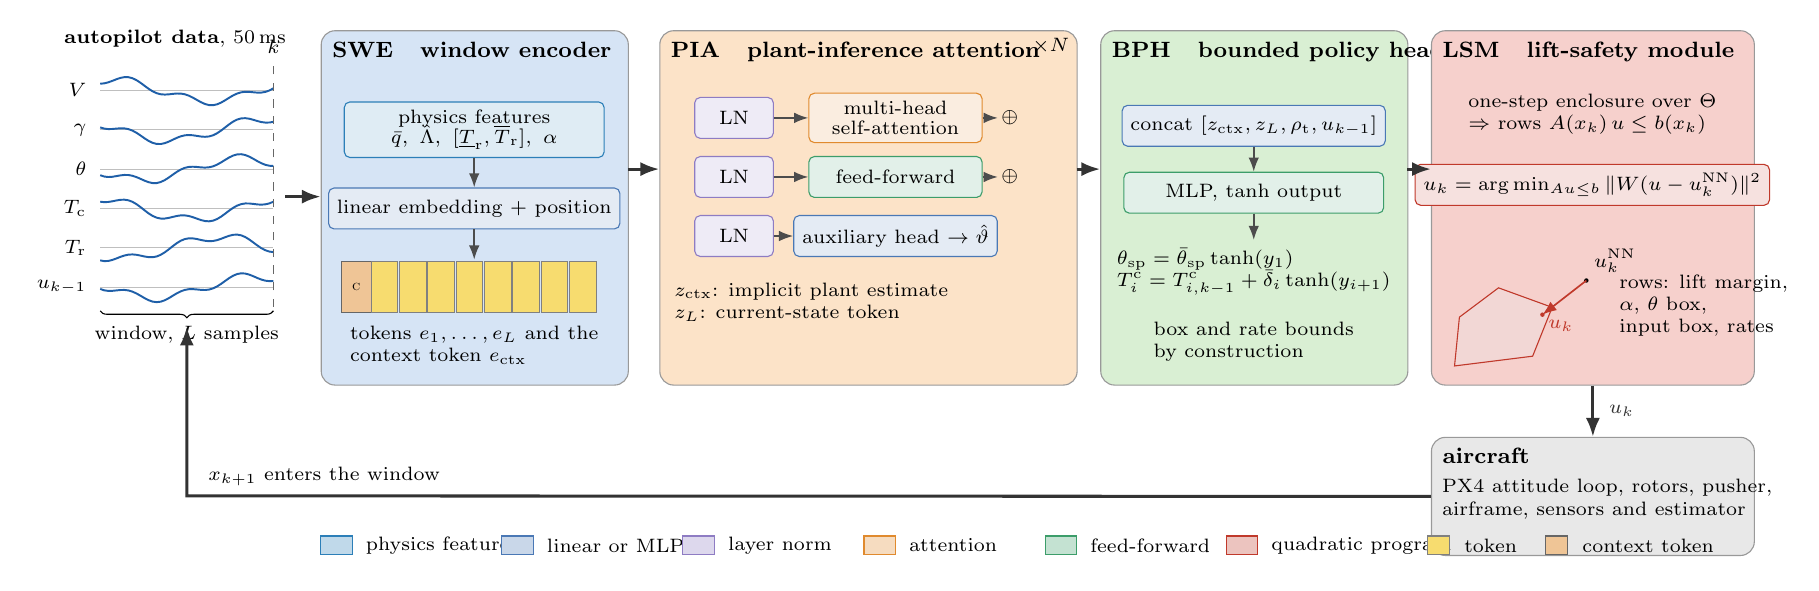
\begin{tikzpicture}[x=1cm,y=1cm]
% ================= measurement window =================
\node[note, anchor=south west] at (0,3.55) {\textbf{autopilot data}, \SI{50}{ms}};
\foreach \i/\nm/\ph in {0/$V$/0, 1/$\gamma$/1.3, 2/$\theta$/2.1, 3/$T_{\mathrm c}$/0.6, 4/$T_{\mathrm r}$/2.8, 5/$u_{k-1}$/1.7}{
  \draw[black!25] (0.5,3.05-0.5*\i) -- (2.7,3.05-0.5*\i);
  \draw[csch, line width=0.7pt, domain=0.5:2.7, samples=44] plot (\x, {3.05-0.5*\i+0.14*sin(2.5*\x r+\ph r)+0.05*sin(9*\x r)});
  \node[font=\scriptsize, anchor=east] at (0.45,3.05-0.5*\i) {\nm};}
\draw[black!60, dashed] (2.7,0.3) -- (2.7,3.4); \node[font=\scriptsize, anchor=south] at (2.7,3.4) {$k$};
\draw[decorate, decoration={brace, amplitude=2.5pt, mirror}] (0.5,0.25) -- (2.7,0.25) node[midway, below=2pt, font=\scriptsize] {window, $L$ samples};
% ================= SWE =================
\node[mod=mSWE, minimum width=3.9cm, minimum height=4.5cm, anchor=south west] (swe) at (3.3,-0.7) {};
\node[modtitle] at (swe.north west) {SWE\quad window encoder};
\node[blk=bPhy, minimum width=33mm] (phys) at (5.25,2.55) {physics features\\[-1pt] $\bar q,\ \hat\Lambda,\ [\underline T_{\mathrm r},\overline T_{\mathrm r}],\ \alpha$};
\node[blk=bLin, minimum width=33mm] (emb) at (5.25,1.55) {linear embedding $+$ position};
\node[ctx] (tctx) at (3.75,0.55) {\textsc{c}};
\foreach \i in {1,...,8}{\node[tok] (t\i) at (3.75+0.36*\i,0.55) {};}
\node[note, anchor=north] at (5.25,0.1) {tokens $e_1,\dots,e_L$ and the\\ context token $e_{\mathrm{ctx}}$};
\draw[arr] (phys) -- (emb); \draw[arr] (emb) -- (5.25,0.9);
\draw[farr] (2.85,1.7) -- (3.3,1.7);
% ================= PIA =================
\node[mod=mPIA, minimum width=5.3cm, minimum height=4.5cm, anchor=south west] (pia) at (7.6,-0.7) {};
\node[modtitle] at (pia.north west) {PIA\quad plant-inference attention};
\node[note, anchor=north east] at (12.85,3.75) {$\times N$};
\foreach \j/\y in {0/2.7,1/1.95,2/1.2}{\node[blk=bLN, minimum width=10mm] (ln\j) at (8.55,\y) {LN};}
\node[blk=bAtt, minimum width=22mm] (att) at (10.6,2.7) {multi-head\\[-1pt] self-attention};
\node[blk=bFFN, minimum width=22mm] (ffn) at (10.6,1.95) {feed-forward};
\node[blk=bLin, minimum width=22mm] (aux) at (10.6,1.2) {auxiliary head $\to\hat\vartheta$};
\draw[arr] (ln0) -- (att); \draw[arr] (ln1) -- (ffn); \draw[arr] (ln2) -- (aux);
\node[font=\scriptsize] at (12.05,2.7) {$\oplus$}; \node[font=\scriptsize] at (12.05,1.95) {$\oplus$};
\draw[arr] (att) -- (11.9,2.7); \draw[arr] (ffn) -- (11.9,1.95);
\node[note, anchor=north west] at (7.75,0.65) {$z_{\mathrm{ctx}}$: implicit plant estimate\\ $z_L$: current-state token};
\draw[farr] (7.2,2.05) -- (7.6,2.05);
% ================= BPH =================
\node[mod=mBPH, minimum width=3.9cm, minimum height=4.5cm, anchor=south west] (bph) at (13.2,-0.7) {};
\node[modtitle] at (bph.north west) {BPH\quad bounded policy head};
\node[blk=bLin, minimum width=33mm] (cat) at (15.15,2.6) {concat $[z_{\mathrm{ctx}},z_L,\rho_{\mathrm t},u_{k-1}]$};
\node[blk=bFFN, minimum width=33mm] (mlp) at (15.15,1.75) {MLP, $\tanh$ output};
\node[note] at (15.15,0.75) {$\thsp=\bar\theta_{\mathrm{sp}}\tanh(y_1)$\\ $T^{\mathrm c}_i=T^{\mathrm c}_{i,k-1}+\bar\delta_i\tanh(y_{i+1})$};
\node[note, anchor=north] at (15.15,0.15) {box and rate bounds\\ by construction};
\draw[arr] (cat) -- (mlp); \draw[arr] (mlp) -- (15.15,1.15);
\draw[farr] (12.9,2.05) -- (13.2,2.05);
% ================= LSM =================
\node[mod=mLSM, minimum width=4.1cm, minimum height=4.5cm, anchor=south west] (lsm) at (17.4,-0.7) {};
\node[modtitle] at (lsm.north west) {LSM\quad lift-safety module};
\node[note] at (19.45,2.75) {one-step enclosure over $\Theta$\\ $\Rightarrow$ rows $A(x_k)\,u\le b(x_k)$};
\node[blk=bQP, minimum width=36mm] (qp) at (19.45,1.85) {$u_k=\arg\min_{Au\le b}\|W(u-u^{\mathrm{NN}}_k)\|^2$};
\begin{scope}[shift={(17.7,-0.45)}, scale=0.62]
\fill[bQP!20, draw=bQP] (0,0) -- (1.6,0.2) -- (2.0,1.2) -- (0.9,1.6) -- (0.1,1.0) -- cycle;
\fill[black] (2.7,1.75) circle (1.3pt) node[font=\scriptsize, above right=-1pt] {$u^{\mathrm{NN}}_k$};
\fill[bQP] (1.8,1.05) circle (1.3pt) node[font=\scriptsize, below right=-2pt] {$u_k$};
\draw[arr, bQP] (2.7,1.75) -- (1.8,1.05);
\end{scope}
\node[note, anchor=north west] at (19.75,0.75) {rows: lift margin,\\ $\alpha$, $\theta$ box,\\ input box, rates};
\draw[farr] (17.1,2.05) -- (17.4,2.05);
% ================= aircraft and loop =================
\node[mod=mPLT, minimum width=4.1cm, minimum height=1.5cm, anchor=north west] (plt) at (17.4,-1.35) {};
\node[modtitle] at (plt.north west) {aircraft};
\node[note, anchor=north west] at (17.5,-1.85) {PX4 attitude loop, rotors, pusher,\\ airframe, sensors and estimator};
\draw[farr] (lsm.south) -- node[right, font=\scriptsize, xshift=2pt] {$u_k$} (plt.north);
\draw[farr] (plt.west) -- (1.6,-2.1) -- (1.6,0.05);
\node[font=\scriptsize, anchor=south west] at (1.75,-2.1) {$x_{k+1}$ enters the window};
% ================= legend =================
\begin{scope}[shift={(3.3,-2.85)}]
\foreach \i/\c/\t in {0/bPhy/physics feature, 1/bLin/linear or MLP, 2/bLN/layer norm, 3/bAtt/attention, 4/bFFN/feed-forward, 5/bQP/quadratic program}{
  \fill[\c!30, draw=\c] (2.3*\i,0) rectangle ++(0.4,0.24); \node[font=\scriptsize, anchor=west] at (2.3*\i+0.45,0.12) {\t};}
\node[tok, minimum height=2.4mm, minimum width=2.8mm] at (14.2,0.12) {}; \node[font=\scriptsize, anchor=west] at (14.4,0.12) {token};
\node[ctx, minimum height=2.4mm, minimum width=2.8mm] at (15.7,0.12) {}; \node[font=\scriptsize, anchor=west] at (15.9,0.12) {context token};
\end{scope}
\end{tikzpicture}
\end{document}
